\documentclass[11pt,a4paper]{article}
\usepackage[margin=1in]{geometry}
\usepackage{graphicx}
\usepackage{booktabs}
\usepackage{hyperref}
\usepackage{enumitem}
\usepackage{tikz}
\usetikzlibrary{arrows.meta, positioning}

\title{ACOP290 C Lab: Spreadsheet Program \\ \large Design Report}
\author{
    % PUT YOUR NAMES AND ENTRY NUMBERS HERE
    Tanvi Parsam (24A1CSEB0022) \and Aditya Murugesh (24A1CSEB0002)
}
\date{\today}

\begin{document}
\maketitle

% ============================================================
\section{Introduction}
% ============================================================

We implemented a command-line spreadsheet program in C that manages a grid of cells ranging from A1 to ZZZ999 (up to 999 rows and 18,278 columns). Each cell holds an integer value, initially 0. Users interact with the program through a REPL interface, setting cell values directly (e.g., \texttt{A1=3}) or via formulas (e.g., \texttt{B1=A1+1}). The spreadsheet supports arithmetic operations, range functions (MIN, MAX, AVG, SUM, STDEV, SLEEP), automatic recalculation of dependent cells, and circular dependency detection. A scrollable 10$\times$10 viewport displays the sheet, and helper commands (\texttt{disable\_output}, \texttt{enable\_output}, \texttt{scroll\_to}) control the display. Running \texttt{make} produces the \texttt{sheet} executable, which is invoked as \texttt{./sheet R C}.

% ============================================================
\section{Program Structure}
% ============================================================

The program is divided into six modules, each in its own source and header file. The diagram below shows how they interact:

\begin{center}
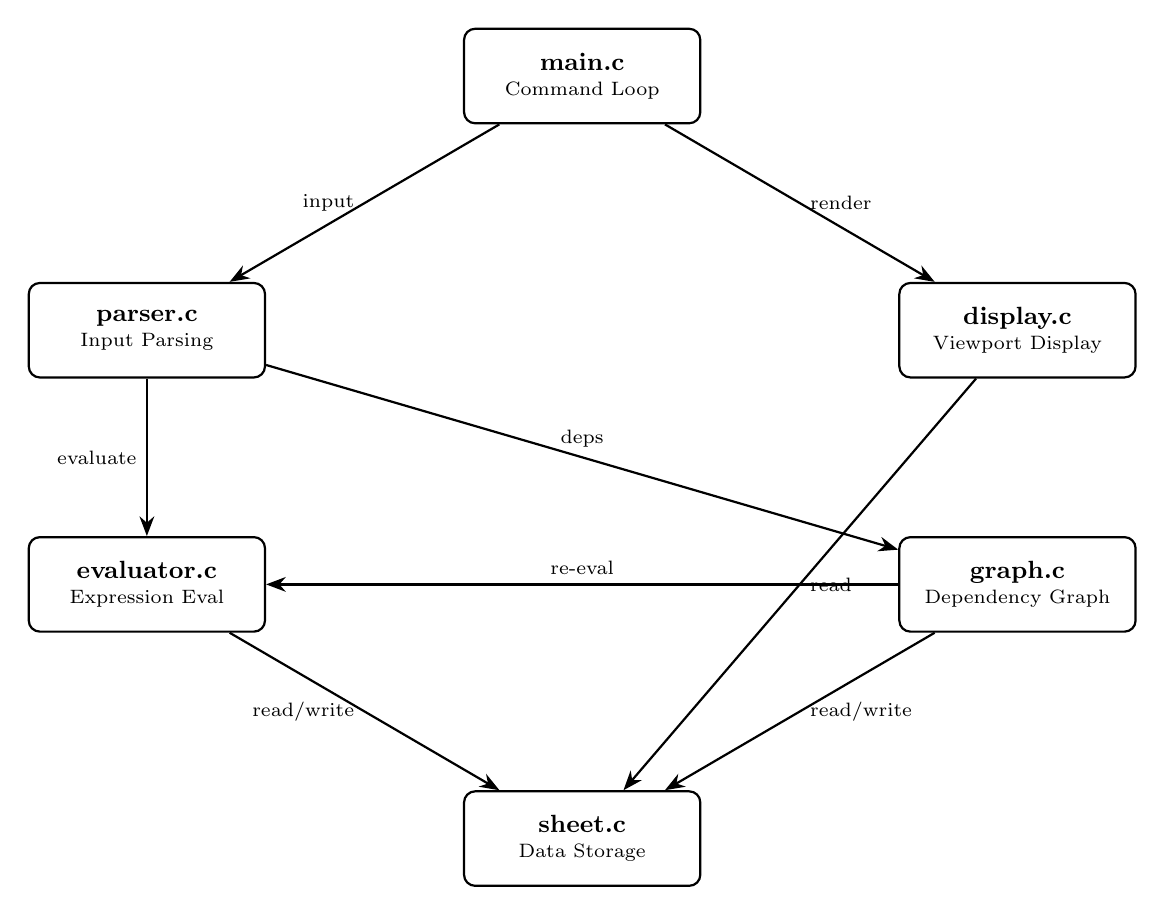
\begin{tikzpicture}[
    module/.style={rectangle, draw, thick, rounded corners, minimum width=3cm, minimum height=1.2cm, align=center, font=\small\bfseries},
    desc/.style={font=\scriptsize, align=center, text width=3cm},
    arrow/.style={-{Stealth[length=2.5mm]}, thick},
    node distance=2cm and 2.5cm
]
    % Nodes
    \node[module] (main) {main.c\\[-2pt]\normalfont\scriptsize Command Loop};
    \node[module, below left=of main] (parser) {parser.c\\[-2pt]\normalfont\scriptsize Input Parsing};
    \node[module, below right=of main] (display) {display.c\\[-2pt]\normalfont\scriptsize Viewport Display};
    \node[module, below=of parser] (eval) {evaluator.c\\[-2pt]\normalfont\scriptsize Expression Eval};
    \node[module, below=of display] (graph) {graph.c\\[-2pt]\normalfont\scriptsize Dependency Graph};
    \node[module, below right=of eval] (sheet) {sheet.c\\[-2pt]\normalfont\scriptsize Data Storage};

    % Arrows
    \draw[arrow] (main) -- node[left, font=\scriptsize]{input} (parser);
    \draw[arrow] (main) -- node[right, font=\scriptsize]{render} (display);
    \draw[arrow] (parser) -- node[left, font=\scriptsize]{evaluate} (eval);
    \draw[arrow] (parser) -- node[above, font=\scriptsize]{deps} (graph);
    \draw[arrow] (eval) -- node[left, font=\scriptsize]{read/write} (sheet);
    \draw[arrow] (graph) -- node[right, font=\scriptsize]{read/write} (sheet);
    \draw[arrow] (graph) -- node[above, font=\scriptsize]{re-eval} (eval);
    \draw[arrow] (display) -- node[right, font=\scriptsize]{read} (sheet);
\end{tikzpicture}
\end{center}

\subsection{Files and Key Functions}

\begin{table}[h]
\centering
\begin{tabular}{@{}lp{4.5cm}p{6cm}@{}}
\toprule
\textbf{File} & \textbf{Purpose} & \textbf{Key Functions} \\
\midrule
sheet.c & Cell storage and coordinate conversion & \texttt{init\_sheet}, \texttt{col\_name\_to\_index}, \texttt{row\_name\_to\_index}, \texttt{index\_to\_col\_name} \\
parser.c & Parse user input into Expression structs & \texttt{parse\_input}, \texttt{parse\_value} \\
evaluator.c & Evaluate expressions, return integer results & \texttt{evaluate}, \texttt{get\_value} \\
graph.c & Dependency tracking, cycle detection, recalculation & \texttt{init\_graph}, \texttt{add\_dependency}, \texttt{clear\_dependency\_graph}, \texttt{has\_circular\_dependency}, \texttt{recalculate\_dependents} \\
display.c & Render 10$\times$10 viewport to terminal & \texttt{print\_sheet} \\
main.c & REPL loop, input routing, timing & \texttt{main} \\
\bottomrule
\end{tabular}
\end{table}

\subsection{Key Data Structures}

\begin{table}[h]
\centering
\begin{tabular}{@{}lp{3cm}p{7cm}@{}}
\toprule
\textbf{Struct} & \textbf{Defined In} & \textbf{Description} \\
\midrule
\texttt{Cell} & sheet.h & Holds an integer \texttt{value}, an \texttt{has\_error} flag, and a \texttt{formula} string (256 bytes) for each cell in the sheet. \\
\texttt{Expression} & parser.h & Represents a parsed formula: its type (constant, cell, arithmetic, function), left/right operands, operator, function type, and range bounds. \\
\texttt{Value} & parser.h & A single operand: either a constant integer (\texttt{is\_cell=0}) or a cell reference with row and column indices (\texttt{is\_cell=1}). \\
\texttt{CellGraphNode} & graph.h & Per-cell graph metadata: a \texttt{dependents} linked list head, a pointer to the stored \texttt{Expression}, and a \texttt{has\_formula} flag. \\
\texttt{DependencyNode} & graph.h & Linked list node for the adjacency list: stores the \texttt{row}, \texttt{col} of a dependent cell and a \texttt{next} pointer. \\
\bottomrule
\end{tabular}
\end{table}

\newpage

% ============================================================
\section{Design Decisions}
% ============================================================

\begin{enumerate}[leftmargin=*]
    \item \textbf{Adjacency list for the dependency graph.} Each cell maintains a linked list of cells that depend on it. When \texttt{B1=A1+1} is entered, B1 is added to A1's dependents list. This is memory-efficient because most cells in a large sheet are independent, so we only allocate memory for actual dependency edges.

    \item \textbf{Heap-allocated stored expressions.} When a formula is set, the parsed \texttt{Expression} is copied to the heap and stored in the graph. During recalculation, cells are re-evaluated directly from this stored expression without re-parsing the formula string, making recalculation fast.

    \item \textbf{Add-then-validate for circular dependencies.} New dependency edges are added to the graph first, then a DFS checks for cycles. If a cycle is detected, the newly added edges are explicitly rolled back. This ensures that the cell's previous valid formula and its dependency edges remain intact on failure.

    \item \textbf{Separate error-check pass for range functions.} Functions like MIN and MAX need an initial value from the first cell in the range. If that cell has an error, the initial value would be garbage. We solve this by scanning the entire range for errors in a first pass before reading any values.

    \item \textbf{Wall-clock timing with \texttt{gettimeofday}.} The C \texttt{clock()} function measures CPU time, so \texttt{SLEEP(2)} would report 0 seconds (the CPU is idle during sleep). Using \texttt{gettimeofday} measures real wall-clock time, correctly reporting 2.0 seconds.
\end{enumerate}

% ============================================================
\section{Challenges Faced}
% ============================================================

\begin{enumerate}[leftmargin=*]
    \item \textbf{Stale dependency edges after failed circular detection.} In an early version, when a circular dependency was detected (e.g., \texttt{A1=MIN(A1:A1)}), the cleanup function could not remove the newly added edges because the expression had not been stored yet. These stale edges remained in the graph, causing subsequent valid commands like \texttt{A1=1} to be falsely flagged as circular. The fix was to explicitly undo the newly added edges using the local expression variable, rather than relying on the stored expression.

    \item \textbf{Destroying old formulas on failed input.} Initially, old dependency edges were cleared before validating the new formula. If the new formula turned out to be circular, the old formula's dependencies were already gone. For example, after \texttt{B1=A1+1} followed by the invalid \texttt{B1=B1+1}, B1 would lose its dependency on A1 and stop recalculating. We fixed this by reordering: old dependencies are only cleared after the new formula passes all validation checks.

    \item \textbf{ERR propagation and recovery.} When a cell transitions to ERR (e.g., \texttt{A1=0} causing \texttt{B2=1/A1} to fail), all downstream dependents must cascade to ERR. When the error source is corrected (\texttt{A1=2}), all those cells must recover their correct values. The recursive \texttt{recalculate\_dependents} function handles both directions naturally by re-evaluating each dependent and propagating further.

    \item \textbf{Memory leak with constant assignments.} Constants are stored with \texttt{has\_formula=0}. The original \texttt{clear\_dependency\_graph} checked this flag first and returned early, skipping the \texttt{free()} call for the stored expression. Repeated constant assignments (e.g., \texttt{A1=1}, \texttt{A1=2}, \texttt{A1=3}) would leak one \texttt{Expression} each time. We fixed this by separating the ``free the expression'' step from the ``remove dependency edges'' step: the expression is always freed, but edges are only removed if the cell had a formula.
\end{enumerate}

\newpage

% ============================================================
\section{Edge Cases and Test Coverage}
% ============================================================

Our test file contains 20 automated tests that verify correct behavior across the following categories:
\begin{table}[h]
\centering
\begin{tabular}{@{}lp{8cm}@{}}
\toprule
\textbf{Category} & \textbf{Test Cases} \\
\midrule
Basic operations & Set constant (\texttt{A1=2}), cell reference (\texttt{B1=A1}), arithmetic (\texttt{A1+3}), integer division truncation (\texttt{5/2=2}) \\
Functions & MIN, MAX, AVG, SUM, STDEV with ranges; SLEEP returns its argument value \\
Ranges & 1D range (\texttt{A1:C1}), 2D range (\texttt{A1:B2}), invalid range where start $>$ end \\
Error handling & Division by zero produces ERR; ERR propagates through dependent cells \\
Dependencies & Single recalculation (\texttt{B1=A1+1}, change A1); chained recalculation across 3 cells \\
Circular deps & Self-reference (\texttt{A1=A1+1}) \\
Boundary checks & Out-of-bounds target cell (\texttt{A3=5} on 2$\times$2 sheet) \\
Helper commands & Unrecognized command shows error; \texttt{disable\_output} suppresses sheet display; \texttt{scroll\_to} with out-of-bounds cell \\
\bottomrule
\end{tabular}
\end{table}

\noindent Tests are run with \texttt{make test}, which compiles \texttt{tests/test.c} and executes it. Each test launches \texttt{./sheet} with the necessary input and checks the output for expected strings.

% ============================================================
\section{Links}
% ============================================================

\begin{itemize}
    \item \textbf{GitHub Repository:} \url{https://github.com/AdityaMurugesh/ACOP290Spreadsheet.git}
\end{itemize}

\end{document}
